% Chapter Template

\chapter{Analysis and Results - Active Monitoring} % Main chapter title

\label{Chapter6} % Change X to a consecutive number; for referencing this chapter elsewhere, use \ref{ChapterX}

\lhead{Chapter 6. \emph{Analysis and Results -  Active Monitoring}} % Change X to a consecutive number; this is for the header on each page - perhaps a shortened title

%----------------------------------------------------------------------------------------
%	SECTION 1
%----------------------------------------------------------------------------------------

%Trying to associate -> rejected some time -> status code = 12 ?
%Connecté et puis disconection abrupte -> code = 3 ?


\section{Analysis}
The purpose of the active monitoring tool is to simulate the behavior of a lambda users that tries to get a connection to the UCL's wireless network in order to access the Internet. In this active monitoring application we have created, as detailed in the implementation and deployment section (see \texttt{4.2.3}), a connection loops in which the supplicant tries to establish a connection with each one of the five UCL's wireless networks. During that loop we also perform an availability and reachability test on a collection of selected services and websites in order to have a better overview of the actual quality and performance of the network the user is experiencing. All the data gathered from these connection loop and tests is inserted into a log file that is sent to the server for parsing and analysis. As a reminder, here are the type of data we store into the log file.

\begin{itemize}
	\item [-] Scan results
	\item [-] APs tried \texttt{BSSIDs}
	\item [-] AP connected to \texttt{BSSID}
	\item [-] Time elapsed during the connection establishment
	\item [-] Time elapsed until an \texttt{IP} address is received from the \texttt{DHCP} server
	\item [-] Services reachability results
\end{itemize}

In this chapter we discuss about the findings we made after having deployed our active monitoring tool on the UCL's network. For each data collected, we detail the results we have and the analysis we can make with them. The limitations we had to face during the development of this application are overview in the last section of this chapter.

% l environnement du router
% genre le signal des point d acces
% tu le pose quelque part et tu vois si la y a des AP avec un bon signal 
% tu dis que c est cool si tu veux voir si la connection d un endroit est bonne toute la journee
% si l environnement RF change etc

\section{Connection Establishment}

\subsection{Scan Results}
The first part of the log file aggregates all the scan results performed by the supplicant before connecting to a network. Those information are quite interesting since they allow us to get live details about the current environment of the router. Thanks to those results we have a full overview of the signal strength of all the surrounding access points as well as their frequencies and the \texttt{SSID} they broadcast. By plotting these information on a graph we are able to make some analysis and conclusion.

On the following graph we can see how the signal of an access point is evolving during the day. 

[INSERT GRAPH HERE]



\subsection{Access Points Interactions}
During the connection establishment phase, the supplicant makes several interactions with the access points. The first interaction they have is in order for the supplicant to associate itself with one of the access points. 


%\subsection{Choice of the Access Point}
%The first thing our program does when it starts its connection loop is to perform a scan of the networks available where the probe is placed and to write the results inside the log file. Among the results and for each network we have decided to keep the network \texttt{BSSID}, the \texttt{Signal Strength} of the network and its \texttt{SSID}. Those data are interesting for our analysis. Indeed, when the router tries to get a connection, it first tries to associate with an Access Point. But there could be several APs in the area and he might be rejected from one or several of them. If its association request is rejected by one AP, \texttt{wpa\_supplicant} will try to associate with another one, and so on until the request is accepted. Our program gathers all the \texttt{BSSID} of the APs it had an association request with. 
%Comparing the scan results for each AP and the APs tried and the one it has a connection with is quite interesting. Indeed, after having performed several tests, we have observed that the device does not always connect to the best AP (i.e. the one with the best signal strength).



\subsubsection*{Access Point Association}

\subsubsection*{Association Rejected}

\subsubsection*{Connection Establishments}

\subsubsection*{Disconnection}




\subsection{Time Durations}
%On peut voir que parfois le temps est plus grand pour se connecter mais ce n'est pas qqch qui revient souvent comme on peut le voir sur le graphique. Les temps de connection et de DHCP sont constants
Time is an important factor when dealing with wireless networks performances. Indeed, the users can be really annoyed when the connection establishment duration begins to take too much time. We have decided to keep track of the time duration it takes for \texttt{wpa\_supplicant} to establish a connection with the network. Conceptually, we start a timer when the command \texttt{SELECT\_NETWORK} is sent to the control interface to start the connection phase and we stop it as soon as a \texttt{WPA-EVENT-CONNECTED} is received. We keep track of the time it takes for the \texttt{DHCP} server to provide an \texttt{IP} address to the supplicant as well. The methodology is the same as the one used for the connection establishment's duration computation. A timer is started as soon as the interface is connected to the network and before sending a \texttt{DISCOVER} message to the \texttt{DHCP} client, and is stopped as soon as a lease for an \texttt{IP} address is obtained.

After gathering some data and plotting it on graphs we have come to conclusion that, despite the fact that we sometimes have peaks in the duration, the connection and \texttt{DHCP} times remain rather constant. Here is an example for the networks \texttt{UCLouvain-prive} and \texttt{UCLouvain}.

\begin{figure}[H]
	\centering
   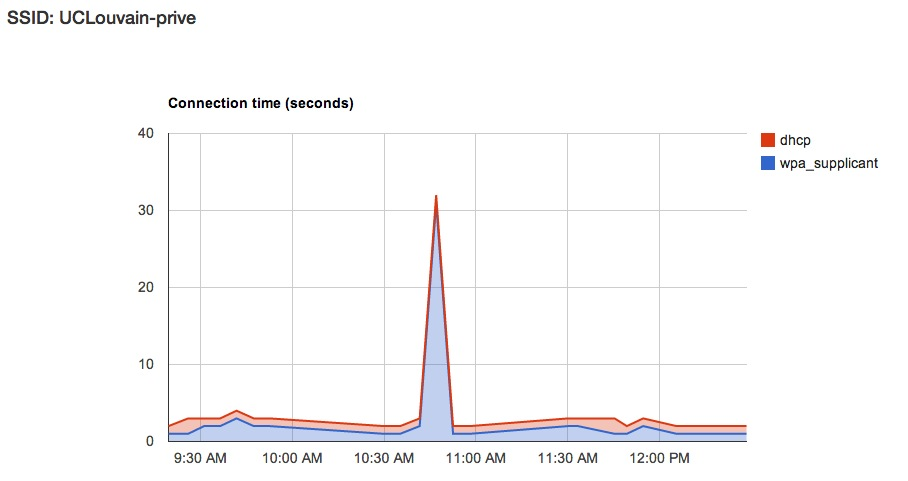
\includegraphics[width=1\textwidth]{Pictures/chapter6/time-uclouvain-prive.jpg}
   \caption{Connection time for \texttt{UCLouvain-prive}}
\end{figure} 

\begin{figure}[H]
	\centering
   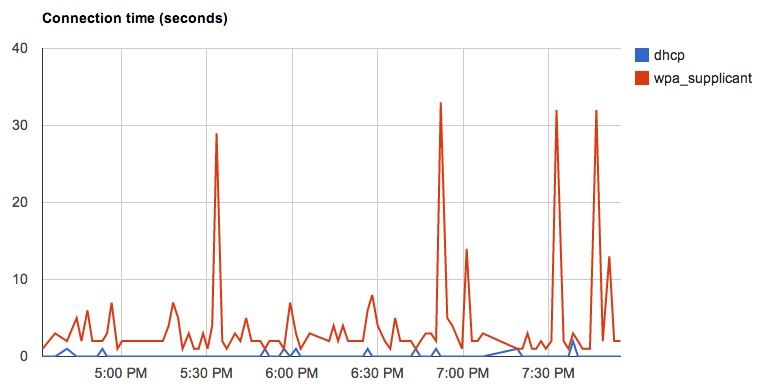
\includegraphics[width=1\textwidth]{Pictures/chapter6/time-uclouvain.jpg}
   \caption{Connection time for \texttt{UCLouvain}}
\end{figure} 

We have investigated on the possible reasons of those peaks and we have noticed that the \texttt{wpa\_supplicant} daemon seems to spend a lot of time in the association phase. Indeed, association with a given AP is sometimes rejected forcing the supplicant to try associate with other ones. This may induce some latency in the connection phase. In order to understand why those rejected association happen, we checked the log file of the \texttt{WiSM} and we found a lot of times the same \texttt{LWAPP} error message.\\

\begin{lstlisting}[frame=single,breaklines=true,caption={\texttt{WiSM} association error message}]
%LWAPP-3-INVALID_AID2: Association identifier [int] for client [hex]:[hex]:[hex]:[hex]:[hex]:[hex] is already in use by[hex]:[hex]:[hex]:[hex]:[hex]:[hex]
\end{lstlisting}

The explanation\footnote{http://www.cisco.com/c/en/us/td/docs/wireless/controller/message/guide/controller\_smg/msgs6.html} \texttt{Cisco} gives for that message is that an internal error caused an invalid association ID to be received from an AP for the indicated client and that the client may experience communications problems.



\section{Services Availability}
We wanted our application to be able to give a performance and quality overview of the network every time a new connection is established. As mentioned before, we have divided our test into two parts. First we perform a \texttt{DNS} query on the two \texttt{DNS} servers of the UCL (with IPs equal to \texttt{130.104.1.1} and \texttt{130.104.1.2}) to see if both servers are reachable. Then we test the \texttt{TCP} connection to the main UCL's services added to the collection of the ten most visited website in the world with simple \texttt{socket} connections. After having received several log files from the router we were able to check the results and make some analysis on them. 

First of all, both \texttt{DNS} servers are always reachable and accessible for the five \texttt{VLANs}. Then, regarding the websites the results depends on which network the test were executed. Indeed, the UCL's online wireless documentation states that some \texttt{VLANs} restrict the range of websites accessible. We were able to confirm that information thanks to the tests we make. Upon our analysis we can see that, only two networks have some restrictions.
\begin{itemize}
	\item [-] \texttt{visiteurs.UCLouvain}
	\item [-] \texttt{UCLouvain-prive}
\end{itemize}





%(sometimes when the daemon gets a connection with an AP for one of the networks it might get abruptly disconnected from that AP but restarts automatically a new connection with another AP for the same network. We keep track of that)








\section{Limitations}
%Limitations ?
%OpenSSL
%Aruba AP70 was originally designed to be a commercial AP instead of a wireless AM, its processing capability is limited: 266-MH MIPS 4Kc CPU, 28-MB RAM, and 8-MB flash memory storage



\section{Summary}
% Signaux
% Temps de connection
% Deconnection

 %https://chromium-review.googlesource.com/#/c/183720/
